\begin{dang}{Xét tính đơn điệu dựa vào BBT và đồ thị}.
\end{dang}
\subsubsection{Các ví dụ}
\begin{vd}%Câu 1.%[Phạm Văn Long]%[2D1Y1-2]
	Cho hàm số $y=f(x)$ có bảng biến thiên như sau: 
	\begin{center}
		\begin{tikzpicture}
		\tikzset{double style/.append style={double distance=1.5pt}}
		\tkzTabInit[nocadre=false,lgt=1.5,espcl=3,deltacl=0.6]
		{$x$ /0.75,$f'(x)$ /0.75,$f(x)$ /2.25}
		{$-\infty$,$2$,$+\infty$}
		\tkzTabLine{,-,d,-,}
		\tkzTabVar{+/$1$,-D+/$-\infty$/$+\infty$,-/$1$}
		\end{tikzpicture}
	\end{center}
	Tìm các khoảng đơn điệu của hàm số $y=f(x)$.
	\loigiai{
		Dựa vào BBT ta có hàm số nghịch biến trên các khoảng $(-\infty;2)$ và $(2;+\infty)$.}
\end{vd}
\begin{vd}%Câu 2.%[Phạm Văn Long]%[2D1B1-2]
	\immini{
		Cho hàm số $f(x)$ xác định trên R và có đồ thị hàm số $y=f'(x)$ là đường cong trong hình bên. Hãy tìm khoảng đồng biến của hàm số trên?
	}{
		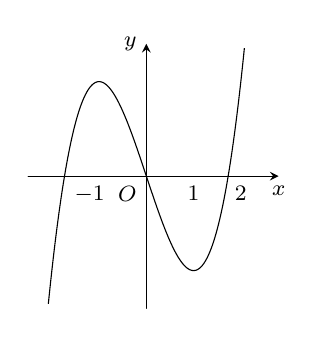
\begin{tikzpicture}[scale=.6,>=stealth, font=\footnotesize, line join=round, line cap=round]
		\def\a{1} \def\b{0} \def\c{-3} \def\d{0} % Hệ số
		\def\xmin{-2.5} \def\xmax{2.8}
		\def\ymin{-2.8} \def\ymax{2.8} 
		\draw[->] (\xmin,0)--(\xmax,0) node [below]{$x$};
		\draw[->] (0,\ymin)--(0,\ymax) node [left]{$y$};
		\node at (0,0) [below left]{$O$};
		\node at (1,0) [below]{$1$};
		\node at (-1.2,0) [below]{$-1$};
		\node at (2,0) [below]{$2$};
		\clip (\xmin+0.1,\ymin+0.1) rectangle (\xmax-0.5,\ymax-0.1);
		\draw[smooth,samples=300] plot(\x,{\a*(\x)^3+\b*(\x)^2+\c*(\x)+\d});
		\end{tikzpicture}
	}	
	\loigiai{
		Dựa vào đồ thị ta có $f'(x)>0,\forall x\in(-1;0)\cup(2;+\infty)$ nên hàm số $f(x)$ đồng biến trên các khoảng $(-1;0)$ và $(2;+\infty)$.}
\end{vd}
\begin{vd}%Câu 3.%[Phạm Văn Long]%[2D1G1-2]
	Cho hàm số $y=f(x)$ có có bảng biến thiên sau: 
	\begin{center}
		\begin{tikzpicture}
		\tkzTabInit[lgt=1.2,espcl=2.5,deltacl=0.6]
		{$x$ /0.6,$y'$ /0.6,$y$ /2}
		{$-\infty$,$-2$,$0$,$2$,$+\infty$}
		\tkzTabLine{,+,$0$,-,$0$,+,$0$,-,}
		\tkzTabVar{-/$-\infty$, +/$3$,-/$-1$,+/$3$,-/$-\infty$}
		\end{tikzpicture}
	\end{center}
	Tìm khoảng nghịch biến của hàm số $y=f\left(x^2-2\right)$?
	\loigiai{
		Từ bảng biến thiên suy ra $f'(x)=0\Leftrightarrow\hoac{&x=0\\&x=\pm 2.}$ \\
		Xét hàm số $y=f\left(x^2-2\right)\Rightarrow y'=2x\cdot f'\left(x^2-2\right)$; $y'=0\Leftrightarrow\hoac{&x=0\\&x^2-2=0\\&x^2-2=\pm 2}\Leftrightarrow\hoac{&x=0\\&x=\pm\sqrt{2}\\&x=\pm 2.}$ \\
		$f'\left(x^2-2\right)>0\Leftrightarrow\hoac{&x^2-2 <-2\\&0<x^2-2<2}\Leftrightarrow\hoac{&-2<x <-\sqrt{2}\\&\sqrt{2}<x<2.}$ \\
		Bảng xét dấu
		\begin{center}
			\begin{tikzpicture}
			\tkzTabInit[lgt=1.2,espcl=2.5,deltacl=0.6]
			{$x$ /0.6,$y'$ /0.6}
			{$-\infty$,$-2$,$-\sqrt2$,$0$,$\sqrt2$,$2$,$+\infty$}
			\tkzTabLine{,+,$0$,-,$0$,+,$0$,-,$0$,+,$0$,-,}
			\end{tikzpicture}
				\end{center}
		Vậy hàm số nghịch biến trên các khoảng $\left(-2;-\sqrt{2}\right)$, $(0;\sqrt{2})$ và $(2;+\infty)$.}
\end{vd}
\begin{vd}%Câu 4.%[Phạm Văn Long]%[2D1G1-2]
	\immini{
		Cho hàm số $f(x)$ có đạo hàm liên tục trên $\mathbb{R}$ và có đồ thị của hàm $y=f'(x)$ như hình vẽ. Tìm các khoảng nghịch biến của hàm số $g(x)=f\left(x^2-2\right)$.
	}{
		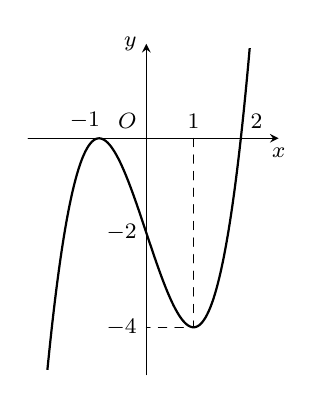
\begin{tikzpicture}[scale=.6,>=stealth, font=\footnotesize, line join=round, line cap=round]
		\def\a{1} \def\b{0} \def\c{-3} \def\d{-2} % Hệ số
		\def\xmin{-2.5} \def\xmax{2.8}
		\def\ymin{-5} \def\ymax{2} 
		\draw[->] (\xmin,0)--(\xmax,0) node [below]{$x$};
		\draw[->] (0,\ymin)--(0,\ymax) node [left]{$y$};
		\draw[dashed] (1,0)--(1,-4)--(0,-4);
		\node at (0,0) [above left]{$O$};
		\node at (1,0) [above]{$1$};
		\node at (-1.3,0) [above]{$-1$};
		\node at (2,0) [above right]{$2$};
		\node at (0,-4) [left]{$-4$};
		\node at (0,-2) [left]{$-2$};
		\clip (\xmin+0.1,\ymin+0.1) rectangle (\xmax-0.5,\ymax-0.1);
		\draw[thick,smooth,samples=300] plot(\x,{\a*(\x)^3+\b*(\x)^2+\c*(\x)+\d});
		\end{tikzpicture}
	}
	\loigiai{
		Ta có $y=g(x)$ là hàm số liên tục trên $\mathbb{R}$ và $g'(x)=2xf'(x^2-2)$. \\
		Nên
		$g'(x)=0\Leftrightarrow\hoac{&x=0\\&x^2-2=-1\\&x^2-2=2}\Leftrightarrow\hoac{&x=0\\&x=\pm 1\\&x=\pm 2.}$ \\
		Từ đồ thị của $y=f'(x)$ suy ra $f'(x^2-2)>0\Leftrightarrow x^2-2>2\Leftrightarrow x\in(-\infty;-2)\cup(2;+\infty)$ và ngược lại. Do đó ta có bảng xét dấu của $g'(x)$: 
		\begin{center}
			\begin{tikzpicture}
			\tkzTabInit[lgt=2.4,espcl=2.3,deltacl=0.6]
			{$x$ /0.6,$x$ /0.6,$f'(x^2-2)$ /0.6,$g'(x)$ /0.6}
			{$-\infty$,$-2$,$-1$,$0$,$1$,$2$,$+\infty$}
			\tkzTabLine{,-,|,-,$|$,-,$0$,+,$|$,+,$|$,+,}
			\tkzTabLine{,+,$0$,-,$0$,-,$|$,-,$0$,-,$0$,+,}
			\tkzTabLine{,-,$0$,+,$0$,+,$0$,-,$0$,-,$0$,+,}
			\end{tikzpicture}
		\end{center}
		Từ BXD ta thấy hàm số $g(x)$ nghịch biến trên các khoảng $(-\infty;-2)$, $(0;1)$ và $(1;2)$
		trên $(-1;0)$ hàm số đồng biến.}
\end{vd}
\subsubsection{Câu hỏi trắc nghiệm}
\Opensolutionfile{ans}[ans/ans2D1-1-2]
\begin{ex}%Câu 1.%[Phạm Văn Long]%[2D1Y1-2]
	Cho hàm số $y=f(x)$ xác định và liên tục trên khoảng $(-\infty;+\infty)$, có bảng biến thiên như hình sau
	\begin{center}
		\begin{tikzpicture}
		\tkzTabInit[lgt=1.2,espcl=2.5,deltacl=0.6]
		{$x$ /0.6,$y'$ /0.6,$y$ /2}
		{$-\infty$,$-1$,$1$,$+\infty$}
		\tkzTabLine{,+,$0$,-,$0$,+,$0$,}
		\tkzTabVar{-/$-\infty$, +/$2$,-/$-1$,+/$+\infty$}
		\end{tikzpicture}
	\end{center}
	Mệnh đề nào sau đây đúng?
	\choice
	{Hàm số nghịch biến trên khoảng $(1;+\infty)$}
	{\True Hàm số đồng biến trên khoảng $(-\infty;-2)$}
	{Hàm số nghịch biến trên khoảng $(-\infty;1)$}
	{Hàm số đồng biến trên khoảng $(-1;+\infty)$}
	\loigiai{
		Từ BBT suy ra hàm số đồng biến trên khoảng $(-\infty;-2)$}
\end{ex}
\begin{ex}%Câu 2.%[Phạm Văn Long]%[2D1Y1-2]
	Cho hàm số $f(x)$ có bảng biến thiên dưới đây. Mệnh đề nào sau đây là sai?
	\begin{center}
		\begin{tikzpicture}
		\tikzset{double style/.append style={double distance=1.5pt}}
		\tkzTabInit[nocadre=false,lgt=1.5,espcl=3,deltacl=0.6]
		{$x$ /0.75,$f'(x)$ /0.75,$f(x)$ /2.25}
		{$-\infty$,$0$,$1$,$+\infty$}
		\tkzTabLine{,-,d,-,0,+,}
		\tkzTabVar{+/$+\infty$,-D+/$-\infty$/$+\infty$,-/$-2$,+/$+\infty$}
		\end{tikzpicture}
	\end{center}
	\choice
	{Hàm số đã cho nghịch biến trên khoảng $(-\infty;0)$}
	{Hàm số đã cho nghịch biến trên khoảng $(0;1)$}
	{\True Hàm số đã cho đồng biến trên khoảng $(0;+\infty)$}
	{Hàm số đã cho đồng biến trên khoảng $(1;+\infty)$}
	\loigiai{
		Từ bảng biên thiên ta thấy trên khoảng $(0;+\infty)$ hàm số nghịch biến trên khoảng $(0;1)$ và đồng biến trên khoảng $(1;+\infty)$. Vậy kết luận hàm số đã cho đồng biến trên khoảng $(0;+\infty)$ là sai.}
\end{ex}
\begin{ex}%Câu 3.%[Phạm Văn Long]%[2D1Y5-1]
	Bảng biến thiên sau là của hàm số nào?
\begin{center}
	\begin{tikzpicture}
	\tikzset{double style/.append style={double distance=1.5pt}}
	\tkzTabInit[nocadre=false,lgt=1.5,espcl=3,deltacl=0.6]
	{$x$ /0.75,$f'(x)$ /0.75,$f(x)$ /2.25}
	{$-\infty$,$2$,$+\infty$}
	\tkzTabLine{,-,d,-,}
	\tkzTabVar{+/$1$,-D+/$-\infty$/$+\infty$,-/$1$}
	\end{tikzpicture}
\end{center}
	\choice
	{$y=\dfrac{2x-1}{x+3}$}
	{$y=\dfrac{4x-6}{x-2}$}
	{$y=\dfrac{3-x}{2-x}$}
	{\True $y=\dfrac{x+5}{x-2}$}
	\loigiai{
		+ Vì $x=2$ là tiệm cận đứng của hàm số nên chọn mẫu $x-2\Rightarrow$ loại ý A\\
		+ Tiệm cận ngang là $y=1$ nên loại ý B\\
		+ $y=\dfrac{3-x}{2-x}=\dfrac{x-3}{x-2};y'=\dfrac{1}{(x-2)^2}>0$ là hàm số đồng biến trên khoảng K $\Rightarrow$ loại C\\
		+ $y=\dfrac{x+5}{x-2};y'=\dfrac{-7}{x-2}<0$ là hàm số nghịch biến trên khoảng K và có tiệm cận đứng $x=2$,tiệm cân ngang $y=1$.}
\end{ex}
\begin{ex}%Câu 4.%[Phạm Văn Long]%[2D1Y1-2]
	Cho hàm số $y=f(x)$ có bảng biến thiên như sau
	\begin{center}
		\begin{tikzpicture}
		\tkzTabInit[lgt=1.2,espcl=2.5,deltacl=0.6]
		{$x$ /0.6,$y'$ /0.6,$y$ /2}
		{$-\infty$,$-1$,$0$,$1$,$+\infty$}
		\tkzTabLine{,-,$0$,+,$0$,-,$0$,+,}
		\tkzTabVar{+/$+\infty$, -/$0$,+/$3$,-/$0$,+/$+\infty$}
		\end{tikzpicture}
	\end{center}
	Mệnh đề nào dưới đây đúng?
	\choice
	{\True Hàm số đồng biến trên các khoảng $(-1;0)$ và $(1;+\infty)$}
	{Hàm số nghịch biến trên các khoảng $(-1;0)$ và $(1;+\infty)$}
	{Hàm số đồng biến trên các khoảng $(0;3)$ và $(0;+\infty)$}
	{Hàm số đồng biến trên các khoảng $(-\infty;-1)$ và $(0;1)$}
	\loigiai{
		Dựa vào bảng biến thiên ta thấy trên khoảng $(-1;0)$ và $(1;+\infty)$ hàm số có $y'>0$ nên hàm số đồng biến trên các khoảng $(-1;0)$ và $(1;+\infty)$.}
\end{ex}
\begin{ex}%Câu 5.%[Phạm Văn Long]%[2D1Y5-1]
	Đường cong hình bên là đồ thị của hàm số có dạng phân thức $y=\dfrac{ax+b}{cx+d}$. Khẳng định nào sau đây đúng?
	\begin{center}
	\begin{tikzpicture}[scale=0.45, font=\footnotesize, line join=round, line cap=round, >=stealth]
	\def\a{1} \def\b{1} \def\c{1} \def\d{-1}
	\def\xmin{-7} \def\xmax{5}
	\def\ymin{-2.3} \def\ymax{6.3}
	\draw[->] (\xmin,0)--(\xmax,0) node [below]{$x$};
	\draw[->] (0,\ymin)--(0,\ymax) node [right]{$y$};
	\node at (0,0) [above left=-3pt]{$O$};
	\clip (\xmin+0.1,\ymin+0.1) rectangle (\xmax-0.1,\ymax-0.1);
	\draw[samples=200,domain=\xmin:(-\d/\c-0.1)] plot(\x,{(\a*(\x)+\b)/(\c*(\x)+\d)});
	\draw[samples=200,domain=(-\d/\c+0.1:\xmax)] plot(\x,{(\a*(\x)+\b)/(\c*(\x)+\d)});
	\draw[dashed] (-\d/\c,\ymin)--(-\d/\c,\ymax);
	\draw[dashed] (\xmin,\a/\c)--(\xmax,\a/\c);
	\draw[fill=black] (1,0) circle (1pt) node[below left=-2pt]{$1$};
	\end{tikzpicture}
\end{center}
	\choice
	{$y'<0,\forall x\in \mathbb{R}$}
	{\True $y'<0,\forall x\neq 1$}
	{$y'>0,\forall x\in \mathbb{R}$}
	{$y'>0,\forall x\neq 1$}
	\loigiai{
		Lý thuyết: Đồ thị hàm số nghịch biến có dạng nhánh từ trái sang phải đi xuống.\\
		Nhìn vào đồ thị ta thấy đây là dạng đồ thị của hàm số nghịch biến trên D và tiệm cận đứng là $x=1$.}
\end{ex}
\begin{ex}%Câu 6.%[Phạm Văn Long]%[2D1Y1-2]
	Cho hàm số $y=f(x)$ có bảng biến thiên sau: 
	\begin{center}
		\begin{tikzpicture}
		\tkzTabInit[lgt=1.2,espcl=2.5,deltacl=0.6]
		{$x$ /0.6,$y'$ /0.6,$y$ /2}
		{$-\infty$,$-1$,$0$,$1$,$+\infty$}
		\tkzTabLine{,-,$0$,+,$0$,-,$0$,+,}
		\tkzTabVar{+/$+\infty$, -/$3$,+/$4$,-/$3$,+/$+\infty$}
		\end{tikzpicture}
	\end{center}
	Các mệnh đề sau đây mệnh đề nào đúng?
	\choice
	{Hàm số đồng biến trên: $(-\infty;0)$ và $(1;+\infty)$}
	{Hàm số nghịch biến trên: $(-\infty;-1)$ và $(1;+\infty)$}
	{\True Hàm số nghịch biến trên: $(-\infty;-1)$ và $(0;1)$}
	{Hàm số đồng biến trên: $(-1;0)$ và $(0;1)$}
	\loigiai{
		Dựa vào BBT, ta thấy hàm số nghịch biến trên: $(-\infty;-1)$ và $(0;1)$; hàm số đồng biến trên: $(-1;0)$ và $(1;+\infty)$.}
\end{ex}
\begin{ex}%Câu 7.%[Phạm Văn Long]%[2D1Y1-2]
	Cho hàm số $y=f(x)$ có bảng biến thiên như hình vẽ dưới đây. 
	\begin{center}
		\begin{tikzpicture}
		\tkzTabInit[lgt=1.2,espcl=2.5,deltacl=0.6]
		{$x$ /0.6,$y'$ /0.6,$y$ /2}
		{$-\infty$,$-2$,$2$,$+\infty$}
		\tkzTabLine{,+,$0$,-,$0$,+,$0$,}
		\tkzTabVar{-/$-\infty$, +/$3$,-/$0$,+/$+\infty$}
		\end{tikzpicture}
	\end{center}
	Hàm số $y=f(x)$ đồng biến trên khoảng nào dưới đây?
	\choice
	{$(-2;2)$}
	{$(-\infty;3)$}
	{$(0;+\infty)$}
	{\True $(2;+\infty)$}
	\loigiai{
		Từ bảng biến thiên ta có hàm số $y=f(x)$ đồng biến trên $(2;+\infty)$.}
\end{ex}
\begin{ex}%Câu 8.%[Phạm Văn Long]%[2D1Y1-2]
	Cho hàm số $y=f(x)$ xác định, liên tục trên $\mathbb{R}$ và có bảng biến thiên sau. Khẳng định nào sau đây đúng?
	\begin{center}
		\begin{tikzpicture}
		\tkzTabInit[lgt=1.2,espcl=2.5,deltacl=0.6]
		{$x$ /0.6,$y'$ /0.6,$y$ /2}
		{$-\infty$,$-1$,$0$,$1$,$+\infty$}
		\tkzTabLine{,-,$0$,+,$0$,-,$0$,+,}
		\tkzTabVar{+/$+\infty$, -/$-1$,+/$0$,-/$-1$,+/$+\infty$}
		\end{tikzpicture}
	\end{center}
	\choice
	{\True Hàm số nghịch biến trên $(-\infty;-1)$ và $(0;1)$}
	{Hàm số nghịch biến trên $(-\infty;-1)$ và $(0;-1)$}
	{Hàm số đạt cực tiểu tại $x=0$}
	{Hàm số đồng biến trên $(-1;+\infty)$}
	\loigiai{
		Hàm số nghịch biến trên $(-\infty;-1)$ và $(0;1)$.\\
		Hàm số đồng biến trên $(-1;0)$ và $(1;+\infty)$.\\
		Hàm số đạt cực đại tại $x=0$.}
\end{ex}
\begin{ex}%Câu 9.%[Phạm Văn Long]%[2D1B1-2]
	Cho hàm số $f(x)$ xác định trên R và có đồ thị hàm số $y=f'(x)$ là đường cong trong hình bên. Mệnh đề nào sau đây là mệnh đề đúng?
\begin{center}
	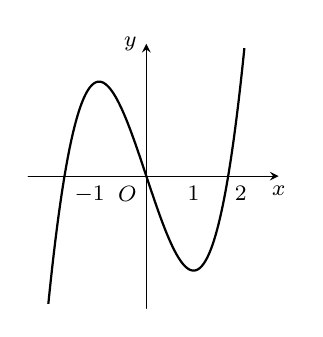
\begin{tikzpicture}[scale=.6,>=stealth, font=\footnotesize, line join=round, line cap=round]
	\def\a{1} \def\b{0} \def\c{-3} \def\d{0} % Hệ số
	\def\xmin{-2.5} \def\xmax{2.8}
	\def\ymin{-2.8} \def\ymax{2.8} 
	\draw[->] (\xmin,0)--(\xmax,0) node [below]{$x$};
	\draw[->] (0,\ymin)--(0,\ymax) node [left]{$y$};
	\node at (0,0) [below left]{$O$};
	\node at (1,0) [below]{$1$};
	\node at (-1.2,0) [below]{$-1$};
	\node at (2,0) [below]{$2$};
	\clip (\xmin+0.1,\ymin+0.1) rectangle (\xmax-0.5,\ymax-0.1);
	\draw[thick,smooth,samples=300] plot(\x,{\a*(\x)^3+\b*(\x)^2+\c*(\x)+\d});
	\end{tikzpicture}
\end{center}
	\choice
	{Hàm số $f(x)$ đồng biến trên $(1;2)$}
	{\True Hàm số $f(x)$ nghịch biến trên $(0;2)$}
	{Hàm số $f(x)$ đồng biến trên $(-2;1)$}
	{Hàm số $f(x)$ nghịch biến trên $(-1;1)$}
	\loigiai{mệnh đề đúng \lq\lq Hàm số $f(x)$ nghịch biến trên $(0;2)$\rq\rq.}
\end{ex}
\begin{ex}%Câu 10.%[Phạm Văn Long]%[2D1G1-2]
	Cho hàm số $f(x)$ có đạo hàm liên tục trên $\mathbb{R}$ và có đồ thị của hàm $y=f'(x)$ như hình vẽ. Xét hàm số $g(x)=f\left(x^2-2\right)$. Mệnh đề nào dưới đây \textbf{sai}?
\begin{center}
	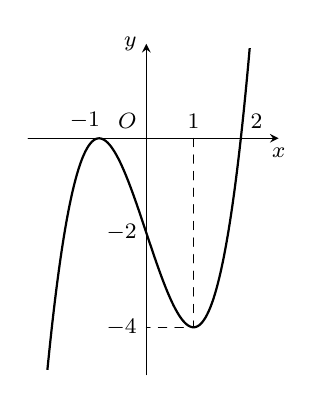
\begin{tikzpicture}[scale=.6,>=stealth, font=\footnotesize, line join=round, line cap=round]
	\def\a{1} \def\b{0} \def\c{-3} \def\d{-2} % Hệ số
	\def\xmin{-2.5} \def\xmax{2.8}
	\def\ymin{-5} \def\ymax{2} 
	\draw[->] (\xmin,0)--(\xmax,0) node [below]{$x$};
	\draw[->] (0,\ymin)--(0,\ymax) node [left]{$y$};
	\draw[dashed] (1,0)--(1,-4)--(0,-4);
	\node at (0,0) [above left]{$O$};
	\node at (1,0) [above]{$1$};
	\node at (-1.3,0) [above]{$-1$};
	\node at (2,0) [above right]{$2$};
	\node at (0,-4) [left]{$-4$};
	\node at (0,-2) [left]{$-2$};
	\clip (\xmin+0.1,\ymin+0.1) rectangle (\xmax-0.5,\ymax-0.1);
	\draw[thick,smooth,samples=300] plot(\x,{\a*(\x)^3+\b*(\x)^2+\c*(\x)+\d});
	\end{tikzpicture}
\end{center}
	\choice
	{Hàm số $g(x)$ nghịch biến trên $(0;2)$}
	{Hàm số $g(x)$ đồng biến trên $(2;+\infty)$}
	{\True Hàm số $g(x)$ nghịch biến trên $(-1;0)$}
	{Hàm số $g(x)$ nghịch biến trên $(-\infty;-2)$}
	\loigiai{
		Ta có $y=g(x)$ là hàm số liên tục trên $\mathbb{R}$ và $g'(x)=2xf'(x^2-2)$. Nên.\\
		$g'(x)=0\Leftrightarrow\hoac{&x=0\\&x^2-2=-1\\&x^2-2=2}\Leftrightarrow\hoac{&x=0\\&x=\pm 1\\&x=\pm 2.}$ \\
		Từ đồ thị của $y=f'(x)$ suy ra $f'(x^2-2)>0\Leftrightarrow x^2-2>2\Leftrightarrow x\in(-\infty;-2)\cup(2;+\infty)$ và ngược lại. Do đó ta có bảng xét dấu của $g'(x)$: 
		\begin{center}
			\begin{tikzpicture}
			\tkzTabInit[lgt=2.5,espcl=2.5,deltacl=0.6]
			{$x$ /0.6,$x$ /0.6,$f'(x^2-2)$ /0.6,$g'(x)$ /0.6}
			{$-\infty$,$-2$,$-1$,$0$,$1$,$2$,$+\infty$}
			\tkzTabLine{,-,|,-,$|$,-,$0$,+,$|$,+,$|$,+,}
			\tkzTabLine{,+,$0$,-,$0$,-,$|$,-,$0$,-,$0$,+,}
			\tkzTabLine{,-,$0$,+,$0$,+,$0$,-,$0$,-,$0$,+,}
			\end{tikzpicture}
		\end{center}
		Từ BXD ta thấy trên $(-1;0)$ hàm số đồng biến. Vậy \lq\lq Hàm số $g(x)$ nghịch biến trên $(-1;0)$\rq\rq\, sai.}
\end{ex}
\begin{ex}%Câu 11.%[Phạm Văn Long]%[2D1Y1-2]
	Cho hàm số $f(x)$ có bảng biến thiên
	\begin{center}
		\begin{tikzpicture}
		\tkzTabInit[lgt=1.2,espcl=2.5,deltacl=0.6]
		{$x$ /0.6,$y'$ /0.6,$y$ /2}
		{$-\infty$,$-1$,$1$,$+\infty$}
		\tkzTabLine{,-,$0$,+,$0$,-,$0$,}
		\tkzTabVar{+/$+\infty$, -/$0$,+/$4$,-/$-\infty$}
		\end{tikzpicture}
	\end{center}
	Chọn khẳng định đúng?
	\choice
	{Hàm số nghịch biến trên $(-1;1)$}
	{Hàm số nghịch biến trên $(-1;+\infty)$}
	{Hàm số đồng biến trên $(-\infty;-1)$}
	{\True Hàm số đồng biến trên $(-1;1)$}
	\loigiai{
		Dựa vào bảng biến thiên ta có trên $(-1;1)$ thì $y'>0$ nên hàm số đồng biến.}
\end{ex}
\begin{ex}%Câu 12.%[Phạm Văn Long]%[2D1Y1-2]
	Cho hàm số $y=f(x)$ xác định và liên tục trên $\mathbb{R}$ và có đồ thị là đường cong trong hình vẽ bên. Mệnh đề nào đúng?
	\begin{center}
		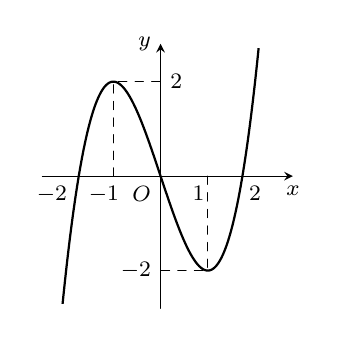
\begin{tikzpicture}[scale=.6,>=stealth, font=\footnotesize, line join=round, line cap=round]
		\def\a{1} \def\b{0} \def\c{-3} \def\d{0} % Hệ số
		\def\xmin{-2.5} \def\xmax{2.8}
		\def\ymin{-2.8} \def\ymax{2.8} 
		\draw[->] (\xmin,0)--(\xmax,0) node [below]{$x$};
		\draw[->] (0,\ymin)--(0,\ymax) node [left]{$y$};
		\draw[dashed] (-1,0)--(-1,2)--(0,2);
		\draw[dashed] (1,0)--(1,-2)--(0,-2);
		\node at (0,0) [below left]{$O$};
		\node at (0.8,0) [below]{$1$};
		\node at (-1.2,0) [below]{$-1$};
		\node at (2,0) [below]{$2$};
		\node at (-2.3,0) [below]{$-2$};
		\node at (0,-2) [left]{$-2$};
		\node at (0,2) [right]{$2$};
		\clip (\xmin+0.1,\ymin+0.1) rectangle (\xmax-0.5,\ymax-0.1);
		\draw[thick,smooth,samples=300] plot(\x,{\a*(\x)^3+\b*(\x)^2+\c*(\x)+\d});
		\end{tikzpicture}
	\end{center}
	\choice
	{Hàm số đồng biến trên khoảng $(-1;1)$}
	{Hàm số nghịch biến trên khoảng $(-2;2)$}
	{\True Hàm số đồng biến trên khoảng $(-\infty;-1)$ và $(1;+\infty)$}
	{Hàm số nghịch biến trên $\mathbb{R}$}
	\loigiai{
		Từ đồ thị ta thấy đồ thị hàm số đi lên (tính từ trái sang phải) trên các khoảng $(-\infty;-1)$ và $(1;+\infty)$.\\
		Suy ra hàm số đồng biến trên khoảng $(-\infty;-1)$ và $(1;+\infty)$.}
\end{ex}
\begin{ex}%Câu 13.%[Phạm Văn Long]%[2D1Y1-2]
	Hàm số $y=x^3-3x+2017$ đồng biến trên khoảng nào?
	\choice
	{\True $(-\infty;-1)$ và $(1;+\infty)$}
	{$(0;+\infty)$}
	{$(-\infty;0)$}
	{$(-\infty;1)$}
	\loigiai{
		Ta có $y'=3x^2-3=0\Leftrightarrow x=\pm 1$.\\
		Bảng biến thiên: 
		\begin{center}
			\begin{tikzpicture}
			\tkzTabInit[lgt=1.2,espcl=2.5,deltacl=0.6]
			{$x$ /0.6,$y'$ /0.6,$y$ /2}
			{$-\infty$,$-1$,$1$,$+\infty$}
			\tkzTabLine{,+,$0$,-,$0$,+,$0$,}
			\tkzTabVar{-/$-\infty$, +/$2019$,-/$2015$,+/$+\infty$}
			\end{tikzpicture}
	\end{center}}
\end{ex}
\begin{ex}%Câu 14.%[Phạm Văn Long]%[2D1Y5-1]
	Trong 4 hàm số sau hàm số nào có bảng biến thiên như hình vẽ?
	\begin{center}
		\begin{tikzpicture}
		\tikzset{double style/.append style={double distance=1.5pt}}
		\tkzTabInit[nocadre=false,lgt=1.5,espcl=3,deltacl=0.6]
		{$x$ /0.75,$f'(x)$ /0.75,$f(x)$ /2.25}
		{$-\infty$,$2$,$+\infty$}
		\tkzTabLine{,-,d,-,}
		\tkzTabVar{+/$1$,-D+/$-\infty$/$+\infty$,-/$1$}
		\end{tikzpicture}
	\end{center}
	\choice
	{$y=\dfrac{x-1}{x+2}$}
	{$y=\dfrac{2x+1}{x-1}$}
	{$y=\dfrac{x-4}{x-2}$}
	{\True $y=\dfrac{x+1}{x-2}$}
	\loigiai{
		Dựa vào bảng biến thiên ta có: phương trình tiệm cận đứng là $x=2$, tiệm cận ngang là $y=1$.\\
		(Loại được đáp án A, B).\\
		Hàm số nghịch biến trên $(-\infty; 2)$ và $(2;+\infty)$ nên C sai vì $y'=\dfrac{2}{(x-2)^2}>0$.\\
		Chọn phương án D vì có đạo hàm $y'=\dfrac{-3}{(x-2)^2}<0\forall x\in \mathscr{D}$.}
\end{ex}
\begin{ex}%Câu 15.%[Phạm Văn Long]%[2D1Y1-2]
	Cho hàm số $y=f(x)$ xác định, liên tục trên $\mathbb{R}$ và có bảng biến thiên:\\
	\begin{center}
		\begin{tikzpicture}
		\tkzTabInit[lgt=1.2,espcl=2.5,deltacl=0.6]
		{$x$ /0.6,$y'$ /0.6,$y$ /2}
		{$-\infty$,$1$,$+\infty$}
		\tkzTabLine{,+,$0$,-,}
		\tkzTabVar{-/$-1$, +/$2$,-/$1$}
		\end{tikzpicture}
	\end{center}
	Mệnh đề nào dưới đây đúng?
	\choice
	{Hàm số đồng biến trên $(-1; 2)$, nghịch biến trên $(1; 2)$}
	{\True Hàm số đồng biến trên $(-\infty; 1)$, nghịch biến trên $(1;+\infty)$}
	{Không thể xác định được khoảng đồng biến, nghịch biến của hàm số}
	{Hàm số nghịch biến trên $(-\infty; 1)$, đồng biến trên $(1;+\infty)$}
	\loigiai{
		Ta có hàm số đồng biến trên $(-\infty; 1)$, nghịch biến trên $(1;+\infty)$.}
\end{ex}
\begin{ex}%Câu 16.%[Phạm Văn Long]%[2D1Y1-2]
	Cho hàm số $y=f(x)$ có bảng xét dấu đạo hàm như sau: 
		\begin{center}
		\begin{tikzpicture}
		\tkzTabInit[lgt=1.2,espcl=2.5,deltacl=0.6]
		{$x$ /0.6,$y'$ /0.6}
		{$-\infty$,$-2$,$0$,$2$,$+\infty$}
		\tkzTabLine{,+,$0$,-,d,-,$0$,-,}
		\end{tikzpicture}
	\end{center}
	Mệnh đề nào dưới đây đúng?
	\choice
	{Hàm số nghịch biến trên khoảng $(-\infty;2)$}
	{Hàm số nghịch biến trên khoảng $(-\infty;-2)$}
	{Hàm số nghịch biến trên khoảng $(-\infty;0)$}
	{\True Hàm số nghịch biến trên khoảng $(-2;0)$}
	\loigiai{
		Hàm số không xác định tại giá trị $0$; trong các đáp án, chỉ có $y'<0,\forall x\in(-2;0)$. Nên mệnh đề đúng là hàm số nghịch biến trên khoảng $(-2;0)$.}
\end{ex}
\begin{ex}%Câu 17.%[Phạm Văn Long]%[2D1Y1-2]
	Cho hàm số $y=f(x)$ có bảng biến thiên như hình vẽ. 
	\begin{center}
		\begin{tikzpicture}
		\tkzTabInit[lgt=1.2,espcl=2.5,deltacl=0.6]
		{$x$ /0.6,$y'$ /0.6,$y$ /2}
		{$-\infty$,$1$,$2$,$+\infty$}
		\tkzTabLine{,+,$0$,-,$0$,+,$0$,}
		\tkzTabVar{-/$-\infty$, +/$3$,-/$0$,+/$+\infty$}
		\end{tikzpicture}
	\end{center}
	Mệnh đề nào sau đây là \textbf{sai}?
	\choice
	{Hàm số đã cho đồng biến trên khoảng $(-\infty;1)$}
	{\True Hàm số đã cho nghịch biến trên khoảng $(0;3)$}
	{Hàm số đã cho đồng biến trên khoảng $(2;+\infty)$}
	{Hàm số đã cho đồng biến trên khoảng $(3;+\infty)$}
	\loigiai{}
\end{ex}
\begin{ex}%Câu 18.%[Phạm Văn Long]%[2D1Y1-2]
	Cho hàm số $y=f(x)$ có đồ thị như hình vẽ bên. 
	\begin{center}
		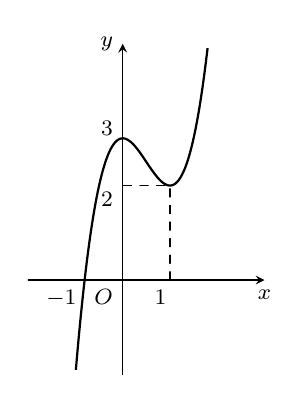
\begin{tikzpicture}[scale=.6,>=stealth, font=\footnotesize, line join=round, line cap=round]
		\def\a{2} \def\b{-3} \def\c{0} \def\d{3} % Hệ số
		\def\xmin{-2} \def\xmax{3}
		\def\ymin{-2} \def\ymax{5} 
		\draw[->] (\xmin,0)--(\xmax,0) node [below]{$x$};
		\draw[->] (0,\ymin)--(0,\ymax) node [left]{$y$};
		\draw[dashed] (1,0)--(1,2)--(0,2);
		\node at (0,0) [below left]{$O$};
		\node at (0.8,0) [below]{$1$};
		\node at (-1.3,0) [below]{$-1$};
		\node at (0,3.2) [left]{$3$};
		\node at (0,1.7) [left]{$2$};
		\clip (\xmin+0.1,\ymin+0.1) rectangle (\xmax-0.5,\ymax-0.1);
		\draw[thick,smooth,samples=300] plot(\x,{\a*(\x)^3+\b*(\x)^2+\c*(\x)+\d});
		\end{tikzpicture}
	\end{center}
	Nhận xét nào sau đây là \textbf{sai}? 
	\choice
	{Hàm số nghịch biến trên khoảng $(0;1)$}
	{Hàm số đạt cực trị tại các điểm $x=0$ và $x=1$}
	{Hàm số đồng biến trên khoảng $(-\infty;0)$ và $(1;+\infty)$}
	{\True Hàm số đồng biến trên khoảng $(-\infty;3)$ và $(1;+\infty)$}
	\loigiai{
		Hàm số đồng biến trên khoảng $(-\infty;3)$ và $(1;+\infty)$.}
\end{ex}
\begin{ex}%Câu 19.%[Phạm Văn Long]%[2D1K1-2]
	Cho hàm số $y=f(x)$ có đạo hàm trên $\mathbb{R}$ thỏa $f(2)=f(-2)=0$ và đồ thị hàm số $y=f'(x)$ có dạng như hình vẽ bên dưới.\\
	\begin{center}
		\begin{tikzpicture}[scale=.6,>=stealth, font=\footnotesize, line join=round, line cap=round]
		\def\a{-1/3} \def\b{1/4} \def\c{1.5} \def\d{-1} % Hệ số
		\def\xmin{-3} \def\xmax{3.5}
		\def\ymin{-2.6} \def\ymax{2} 
		\draw[->] (\xmin,0)--(\xmax,0) node [below]{$x$};
		\draw[->] (0,\ymin)--(0,\ymax) node [left]{$y$};
		\draw[dashed] (-1,0)--(-1,-23/12)--(0,-23/12);
		\draw[dashed] (1.5,0)--(1.5,11/16)--(0,11/16);
		\node at (0,0) [below left]{$O$};
		\node at (0.8,0) [below]{$1$};
		\node at (-2.7,0) [below]{$-2$};
		\node at (2.7,0) [below]{$2$};
		\node at (-1.5,0) [below]{$-1$};
		\node at (1.5,0) [below]{$\dfrac{3}{2}$};
		\clip (\xmin+0.1,\ymin+0.1) rectangle (\xmax-0.5,\ymax-0.1);
		\draw[thick,smooth,samples=300] plot(\x,{\a*(\x)^3+\b*(\x)^2+\c*(\x)+\d});
		\end{tikzpicture}
	\end{center}
	Hàm số $y=\left(f(x)\right)^2$ nghịch biến trên khoảng nào trong các khoảng sau: 
	\choice
	{$\left(-1;\dfrac{3}{2}\right)$}
	{$(-2;-1)$}
	{$(-1;1)$}
	{\True $(1;2)$}
	\loigiai{
		Dựa vào đồ thị hàm số $y=f'(x)$ ta lập được bảng biến thiên của $y=f(x)$ như sau: 
		\begin{center}
			\begin{tikzpicture}
			\tkzTabInit[lgt=1.2,espcl=2.5,deltacl=0.6]
			{$x$ /0.6,$y'$ /0.6,$y$ /2}
			{$-\infty$,$-2$,$1$,$2$,$+\infty$}
			\tkzTabLine{,+,$0$,-,$0$,+,$0$,-,}
			\tkzTabVar{-/$-\infty$, +/$0$,-/$ $,+/$0$,-/$-\infty$}
			\end{tikzpicture}
		\end{center}
		Dựa vào bảng biến thiên ta thấy $f(x)\leq 0,\forall x\in\mathbb{R}$.\\
		Xét hàm số $y=\left(f(x)\right)^2$, ta có $y'=2f(x)\cdot f'(x)$.\\
		Tìm khoảng để hàm số $y=\left(f(x)\right)^2$ nghịch biến nên ta cần tìm $x$ để $y'\leq 0$.\\
		Do $f(x)\leq 0,\forall x\in\mathbb{R}$ nên $y'\leq 0\Leftrightarrow f'(x)\geq 0\Leftrightarrow\hoac{&x\leq-2\\&1\leq x\leq 2.}$ \\
		Do đó hàm số $y=\left(f(x)\right)^2$ nghịch biến trên khoảng $(-\infty;-2)$ và $(1;2)$.}
\end{ex}
\begin{ex}%Câu 20.%[Phạm Văn Long]%[2D1G1-2]
	Hàm số $y=f(x)$ có đồ thị $y=f'(x)$ như hình vẽ. 
	\begin{center}
		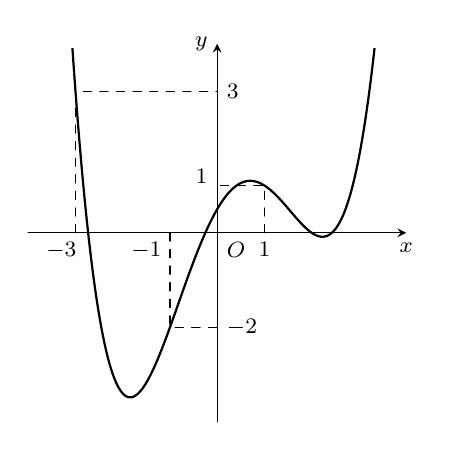
\begin{tikzpicture}[scale=.6,>=stealth, font=\footnotesize, line join=round, line cap=round]
		\def\a{3/20} \def\b{-13/60} \def\c{-23/20} \def\d{103/60} \def\e{0.5} % Hệ số
		\def\xmin{-4} \def\xmax{4}
		\def\ymin{-4} \def\ymax{4} 
		\draw[->] (\xmin,0)--(\xmax,0) node [below]{$x$};
		\draw[->] (0,\ymin)--(0,\ymax) node [left]{$y$};
		\draw[dashed] (-3,0)--(-3,3)--(0,3);
		\draw[dashed] (-1,0)--(-1,-2)--(0,-2);
		\draw[dashed] (1,0)--(1,1)--(0,1);
		\node at (0,0) [below right]{$O$};
		\node at (1,0) [below]{$1$};
		\node at (0,-2) [right]{$-2$};
		\node at (0,1.2) [left]{$1$};
		\node at (0,3) [right]{$3$};
		\node at (-1.5,0) [below]{$-1$};
		\node at (-3.3,0) [below]{$-3$};
		\clip (\xmin+0.1,\ymin+0.1) rectangle (\xmax-0.5,\ymax-0.1);
		\draw[thick,smooth,samples=300] plot(\x,{\a*(\x)^4+\b*(\x)^3+\c*(\x)^2+\d*(\x)+\e});
		\end{tikzpicture}
	\end{center}
	Xét hàm số $g(x)=f(x)-\dfrac{1}{3}x^3-\dfrac{3}{4}x^2+\dfrac{3}{2}x+2017$.\\
	Nhận xét nào sau đây là sai: 
	\choice
	{Hàm số $g(x)$ nghịch biến trên $(-3;-1)$}
	{Hàm số nghịch biến trên khoảng $(1;+\infty)$}
	{Hàm số đồng biến trên khoảng $(-1;1)$}
	{\True Hàm số $g(x)$ đồng biến trên $(-3;-1)$}
	\loigiai{
		$g'(x)=f'(x)-\left(x^2+\dfrac{3}{2}x-\dfrac{3}{2}\right)$.\\
		Trên mặt phẳng toạ độ đã có đồ thị hàm số $f'(x)$ ta vẽ thêm đồ thị hàm số $y=x^2+\dfrac{3}{2}x-\dfrac{3}{2}$. 
	\begin{center}
		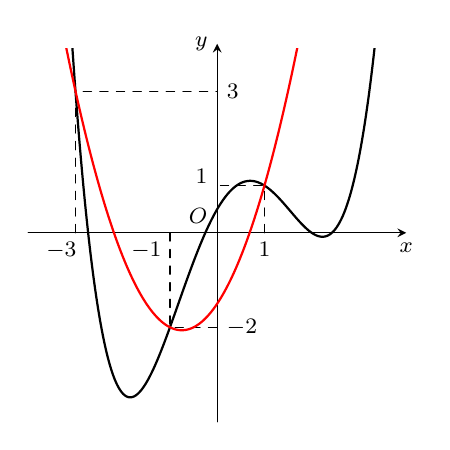
\begin{tikzpicture}[scale=.6,>=stealth, font=\footnotesize, line join=round, line cap=round]
		\def\a{3/20} \def\b{-13/60} \def\c{-23/20} \def\d{103/60} \def\e{0.5} % Hệ số
		\def\xmin{-4} \def\xmax{4}
		\def\ymin{-4} \def\ymax{4} 
		\draw[->] (\xmin,0)--(\xmax,0) node [below]{$x$};
		\draw[->] (0,\ymin)--(0,\ymax) node [left]{$y$};
		\draw[dashed] (-3,0)--(-3,3)--(0,3);
		\draw[dashed] (-1,0)--(-1,-2)--(0,-2);
		\draw[dashed] (1,0)--(1,1)--(0,1);
		\node at (0,0) [above left]{$O$};
		\node at (1,0) [below]{$1$};
		\node at (0,-2) [right]{$-2$};
		\node at (0,1.2) [left]{$1$};
		\node at (0,3) [right]{$3$};
		\node at (-1.5,0) [below]{$-1$};
		\node at (-3.3,0) [below]{$-3$};
		\clip (\xmin+0.1,\ymin+0.1) rectangle (\xmax-0.5,\ymax-0.1);
		\draw[thick,smooth,samples=300] plot(\x,{\a*(\x)^4+\b*(\x)^3+\c*(\x)^2+\d*(\x)+\e});
		\draw[thick,smooth,red,samples=300] plot(\x,{(\x)^2+1.5*(\x)-1.5});
		\end{tikzpicture}
	\end{center}
		Dựa vào đồ thị hàm số ta có\\
		Khi $x\in(-3;-1)$ thì $f'(x)<x^2+\dfrac{3}{2}x-\dfrac{3}{2}$, do đó $g'(x)<0,\forall x\in(-3;-1)$.\\
		Suy ra hàm số $g(x)$ nghịch biến trên $(-3;-1)$.\\
		là hàm số đồng biến trên các khoảng $(-\infty;-3)$ và $(-3;+\infty)$.}
\end{ex}
\Closesolutionfile{ans}